\section{Regla de Centralidad-Letalidad}
En el trabajo de de \citet{jeong2000} se establece una correlaci\'on entre esencialidad y los hubs de una red metab\'olica. 
Esta correlaci\'on ha sido llamada \textit{Regla de Centralidad-Letalidad} y ha sido reportada en otros trabajos 
citep{yu2004,winzeler1999,wuchty2002}. En \citet{jeong2000} se explora la posibilidad de estimar la esencialidad de un
nodo a partir de la centralidad por grado. En esta secci\'on veremos que si bien si existe una correlaci\'on entre esencilidad y los hubs, el comportamiento de estos ultimos (e incluso nodos centrales por otras medidas) no se corresponde con el de un 
nodo esencial.

\subsection{Cumplimiento de la regla}
Utilizando una lista de 1155 proteinas esenciales de levadura, se busca la relaci\'on entre esencialidad y alto grado de un nodo, donde \textit{alto grado (hub)} debe ser definido. La figura \ref{fig:esshub} muestra esta relaci\'on: en el eje horizontal el 
porcentaje de nodos que son considerados hubs, y en el eje vertical la fracc\'ion de nodos esencialides que adem\'as son hubs. 
De la figura se puede ver que el caso de la red Y2H los nodos esenciales estan repartidos homogeniamente en los distintos grados, mientras que el resto de las redes diluye a los escenciales con el aumento del umbral que define a los hubs, es decir, los nodos 
esenciales de estas redes se encuentran, principalmente, entre los hubs de mayor grado.

\begin{figure}[!ht]
    \centering
    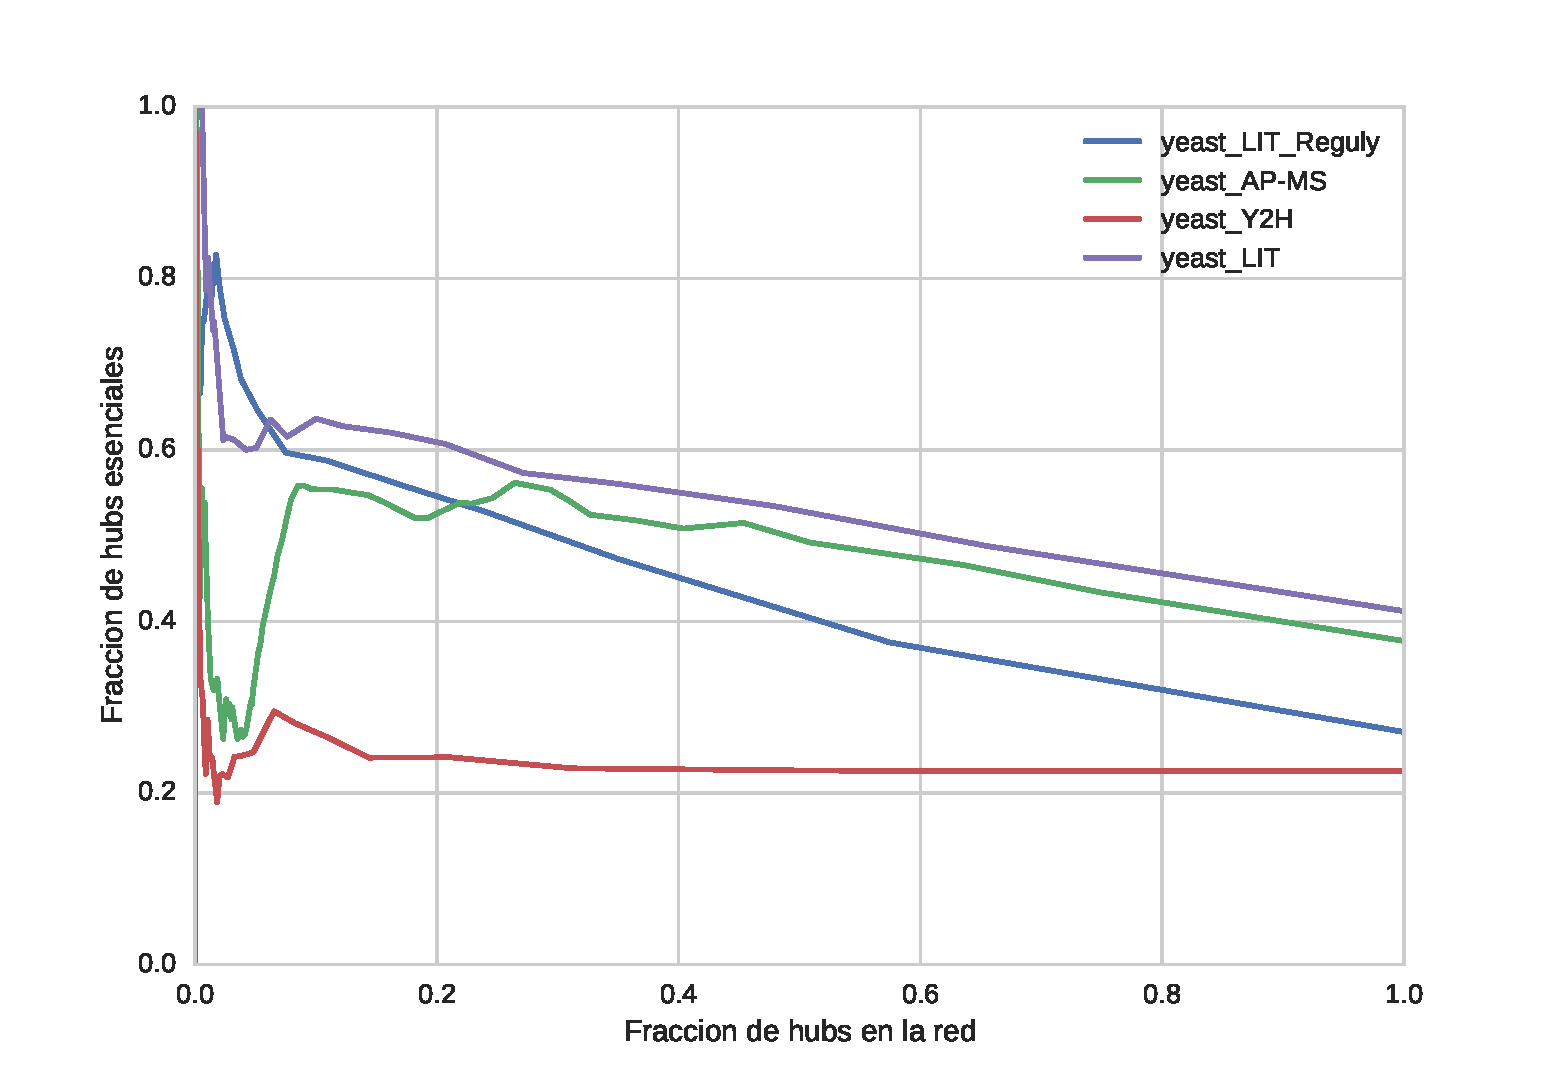
\includegraphics[width=.8\columnwidth]{./schemes/ess_hub.pdf}
    \caption{\label{fig:esshub} Fracci\'on de hubs esenciales en funci\'on de fracci\'on de hubs en relaci\'on al total de nodos de la red.  }
\end{figure}


La tabla \ref{tab:cl} muestra los indices de correlaci\'on de Kendall ($\tau$) y de Spearman ($\rho$) de esencialidad con fracci\'on de hubs en la red. Se puede apreciar que incluso para diferentes umbrales de definici\'on de hub, existe una significativa
correlaci\'on (tanto de Kendall como de Spearman)
entre estas dos caracteristicas; As\'i tambien se puede ver que debido a las distintas conectividades de la redes, los grados, 
a partir de los cuales definimos hub, son muy distintos para cada red.


\begin{table}[!ht]
    \centering
    \caption{\label{tab:cl}Indices de correlaci\'on de Rendall ($\tau$) y Spearman ($\rho$), con sus respectivos $p_\text{valor}$, para relaci\'on entre esencialidad y 
grado de un nodo para dos definiciones porcentuales de hubs respecto al total de la red ( $\sim10\%$ y $\sim20\%$ de los nodos son hubs).}
    {\scriptsize
    \begin{tabularx}{.8\columnwidth}{XcX|XcccX}
        \hline\hline
        &               &&& \multicolumn{3}{c}{$\% 10$ de corte }             \\ 
        \cline{5-7}
        &               &&& $\tau$ &        $\rho$          & $k_{cut}$     \\
        \hline
        & AP-MS         &&& 0.62(6.5e-13) & 0.70(1.3e-10) & 27           \\ 
        & LIT           &&& 0.89(1.4e-08) & 0.94(2.4e-10) & 9             \\
        & Y2H           &&& 0.72(4.3e-08) & 0.79(3.8e-07) & 6             \\
        & LIT\_Reguly   &&& 0.84(2.3e-19)   & 0.91(5.0e-22) & 16          \\
        \hline
        &               &&& \multicolumn{3}{c}{$\% 20$ de corte} & \\
        \cline{5-7}
        &               &&& $\tau$        & $\rho$ & $k_{cut}$ &  \\
        \hline
        & AP-MS         &&&0.72(2.7e-19) & 0.81(1.4e-17) & 18 \\
        & LIT           &&&0.92(2.7e-10) & 0.96(9.6e-14) & 6  \\
        & Y2H           &&&0.75(2.5e-09) & 0.84(8.2e-09) & 4  \\
        & LIT\_Reguly   &&&0.88(4.9e-23) & 0.94(2.2e-28) & 10  \\
        \hline\hline
    \end{tabularx}
    }
\end{table}
